\documentclass[11pt]{article}

\usepackage[margin=1in]{geometry}
\usepackage{amsmath, amssymb, amsthm}
\usepackage{enumitem}
\usepackage{tikz}

\pagestyle{empty}

\begin{document}

\begin{center}
  {\Large\bfseries Weekly Assignment: Graphs and the Handshake Theorem (Epp~1.4 \& 4.9)}
\end{center}

\bigskip

\noindent
Complete each of the following problems.  Show all work and justify your answers.

\bigskip

%% ─────────────────────────────────────────────
\noindent\textbf{Problem 1} (Epp 1.4 \#4). \;
Draw a picture of graph~$H$, which has vertex set
$\{v_1, v_2, v_3, v_4, v_5\}$ and edge set $\{e_1, e_2, e_3, e_4\}$
with the following edge-endpoint function:

\medskip
\begin{center}
\begin{tabular}{c|c}
\textbf{Edge} & \textbf{Endpoints} \\ \hline
$e_1$ & $\{v_1\}$ \\
$e_2$ & $\{v_2, v_3\}$ \\
$e_3$ & $\{v_2, v_3\}$ \\
$e_4$ & $\{v_1, v_5\}$
\end{tabular}
\end{center}

\bigskip

%% ─────────────────────────────────────────────
\noindent\textbf{Problem 2} (Epp 1.4 \#6). \;
Show that the two drawings represent the same graph by labeling the
vertices and edges of drawing~(b) to correspond to those of drawing~(a).

\begin{center}
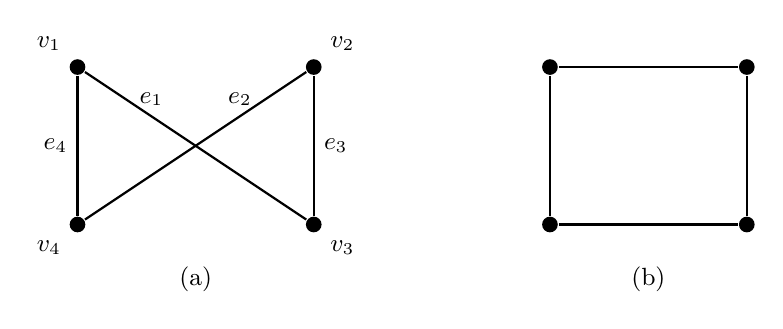
\begin{tikzpicture}[
    vertex/.style={circle, fill=black, inner sep=2pt},
    every node/.style={font=\small},
    thick
  ]
  % --- Drawing (a) ---
  \node[vertex, label=above left:$v_1$] (v1) at (0,2) {};
  \node[vertex, label=above right:$v_2$] (v2) at (3,2) {};
  \node[vertex, label=below right:$v_3$] (v3) at (3,0) {};
  \node[vertex, label=below left:$v_4$] (v4) at (0,0) {};

  % e4: v1 -- v4 (left side)
  \draw (v1) -- node[left] {$e_4$} (v4);
  % e3: v2 -- v3 (right side)
  \draw (v2) -- node[right] {$e_3$} (v3);
  % e1: v1 -- v3 (diagonal)
  \draw (v1) -- node[above, pos=0.3] {$e_1$} (v3);
  % e2: v2 -- v4 (diagonal)
  \draw (v2) -- node[above, pos=0.3] {$e_2$} (v4);

  \node at (1.5,-0.7) {(a)};

  % --- Drawing (b) ---
  \begin{scope}[xshift=6cm]
    \node[vertex] (a) at (0,2) {};
    \node[vertex] (b) at (2.5,2) {};
    \node[vertex] (c) at (2.5,0) {};
    \node[vertex] (d) at (0,0) {};

    \draw (a) -- (b);
    \draw (b) -- (c);
    \draw (c) -- (d);
    \draw (a) -- (d);

    \node at (1.25,-0.7) {(b)};
  \end{scope}
\end{tikzpicture}
\end{center}

\bigskip

%% ─────────────────────────────────────────────
\noindent\textbf{Problem 3} (Epp 4.9 \#8). \;
Either draw a graph with four vertices of degrees 1, 2, 3, and 4,
or explain why no such graph exists.

\bigskip

%% ─────────────────────────────────────────────
\noindent\textbf{Problem 4} (Epp 4.9 \#13). \;
Either draw a simple graph with nine edges and all vertices of degree~3,
or explain why no such graph exists.

\bigskip

%% ─────────────────────────────────────────────
\noindent\textbf{Problem 5} (Epp 4.9 \#15). \;
A small social network contains three people who are network friends with
six other people in the network, one person who is network friends with
five other people in the network, and five people who are network friends
with four other people in the network.  The rest are network friends with
three other people in the network.  The network contains 41 pairs of
network friends.
\begin{enumerate}[label=\alph*.]
  \item How many people are network friends with three other people
        in the network?
  \item How many people are in the network?
\end{enumerate}

\bigskip

%% ─────────────────────────────────────────────
\noindent\textbf{Problem 6} (Epp 4.9 \#20).
\begin{enumerate}[label=\alph*.]
  \item Draw $K_6$, a complete graph on six vertices.
  \item Use the result of Example~4.9.9 to show that the number of edges
        of a simple graph with $n$ vertices is less than or equal to
        $\displaystyle\frac{n(n-1)}{2}$.
\end{enumerate}

\bigskip

%% ─────────────────────────────────────────────
\noindent\textbf{Problem 7} (Puzzle). \;
A couple \emph{really} wants to have a baby girl.  They decide to have
children until they have a girl, but realistically they will give up if
they have four consecutive boys.  Assume each child is independently
equally likely to be a boy or a girl.

\medskip
What is the expected number of boys and the expected number of girls
in their family?

\medskip\noindent
\emph{Hint}: List every possible outcome and its probability, then compute
the expectations directly.

\end{document}
